\documentclass[a4paper,10pt,twocolumn,oneside]{article}
\setlength{\columnsep}{10pt}                    %兩欄模式的間距
\setlength{\columnseprule}{0pt}                 %兩欄模式間格線粗細

\usepackage{amsthm}                             %定義，例題
\usepackage{amssymb}
\usepackage{fontspec}                           %設定字體
\usepackage{color}
\usepackage[x11names]{xcolor}
\usepackage{listings}                           %顯示code用的
\usepackage{fancyhdr}                           %設定頁首頁尾
\usepackage{graphicx}                           %Graphic
\usepackage{enumerate}
\usepackage{titlesec}
\usepackage{amsmath}
\usepackage[CheckSingle, CJKmath]{xeCJK}
\usepackage{CJKulem}
\usepackage{tikz}

\titlespacing{\section}{0cm}{0cm}{0cm}
\titlespacing{\subsection}{0cm}{0cm}{0cm}
\usepackage{amsmath, courier, listings, fancyhdr, graphicx}
\topmargin=0pt
\headsep=5pt
\textheight=780pt
\footskip=0pt
\voffset=-55pt
\textwidth=560pt
\marginparsep=0pt
\marginparwidth=0pt
\marginparpush=0pt
\oddsidemargin=0pt
\evensidemargin=0pt
\hoffset=-55pt

%\renewcommand\listfigurename{圖目錄}
%\renewcommand\listtablename{表目錄}

%%%%%%%%%%%%%%%%%%%%%%%%%%%%%

\setmainfont[
    AutoFakeSlant,
    BoldItalicFeatures={FakeSlant},
    UprightFont={* Medium},
    BoldFont={* Bold}
]{Inconsolata}
%\setmonofont{Ubuntu Mono}
\setmonofont[
    AutoFakeSlant,
    BoldItalicFeatures={FakeSlant},
    UprightFont={* Medium},
    BoldFont={* Bold}
]{Inconsolata}
\setCJKmainfont{Noto Sans CJK TC}
\XeTeXlinebreaklocale "zh"                      %中文自動換行
\XeTeXlinebreakskip = 0pt plus 1pt              %設定段落之間的距離
\setcounter{secnumdepth}{3}                     %目錄顯示第三層

%%%%%%%%%%%%%%%%%%%%%%%%%%%%%
\makeatletter
\lst@CCPutMacro\lst@ProcessOther {"2D}{\lst@ttfamily{-{}}{-{}}}
\@empty\z@\@empty
\makeatother
\lstset{                                        % Code顯示
    language=C++,                               % the language of the code
    basicstyle=\normalsize\ttfamily,          % the size of the fonts that are used for the code
    numbers=left,                               % where to put the line-numbers
    columns=fixed,
    basewidth=0.48em,
    numberstyle=\tiny,                    % the size of the fonts that are used for the line-numbers
    stepnumber=1,                               % the step between two line-numbers. If it's 1, each line  will be numbered
    numbersep=5pt,                              % how far the line-numbers are from the code
    backgroundcolor=\color{white},              % choose the background color. You must add \usepackage{color}
    showspaces=false,                           % show spaces adding particular underscores
    showstringspaces=false,                     % underline spaces within strings
    showtabs=false,                             % show tabs within strings adding particular underscores
    frame=false,                                % adds a frame around the code
    tabsize=2,                                  % sets default tabsize to 2 spaces
    captionpos=b,                               % sets the caption-position to bottom
    breaklines=true,                            % sets automatic line breaking
    breakatwhitespace=true, % sets if automatic breaks should only happen at whitespace
    escapeinside={\%*}{*)},                     % if you want to add a comment within your code
    morekeywords={*},                           % if you want to add more keywords to the set
    keywordstyle=\bfseries\color{Blue1},
    commentstyle=\itshape\color{Red1},
    stringstyle=\itshape\color{Green4},
}


\begin{document}
\pagestyle{fancy}
\fancyfoot{}
%\fancyfoot[R]{\includegraphics[width=20pt]{ironwood.jpg}}
\fancyhead[C]{CodeBook}
\fancyhead[L]{singhone0515}
\fancyhead[R]{\thepage}
\renewcommand{\headrulewidth}{0.4pt}
\renewcommand{\contentsname}{Contents}

\newcommand{\includetex}[2]{
  \subsection{#1}
  \input{#2}
  \vspace{-1.2em}
}
\newcommand{\gridpage}{
    \clearpage
    \centering
    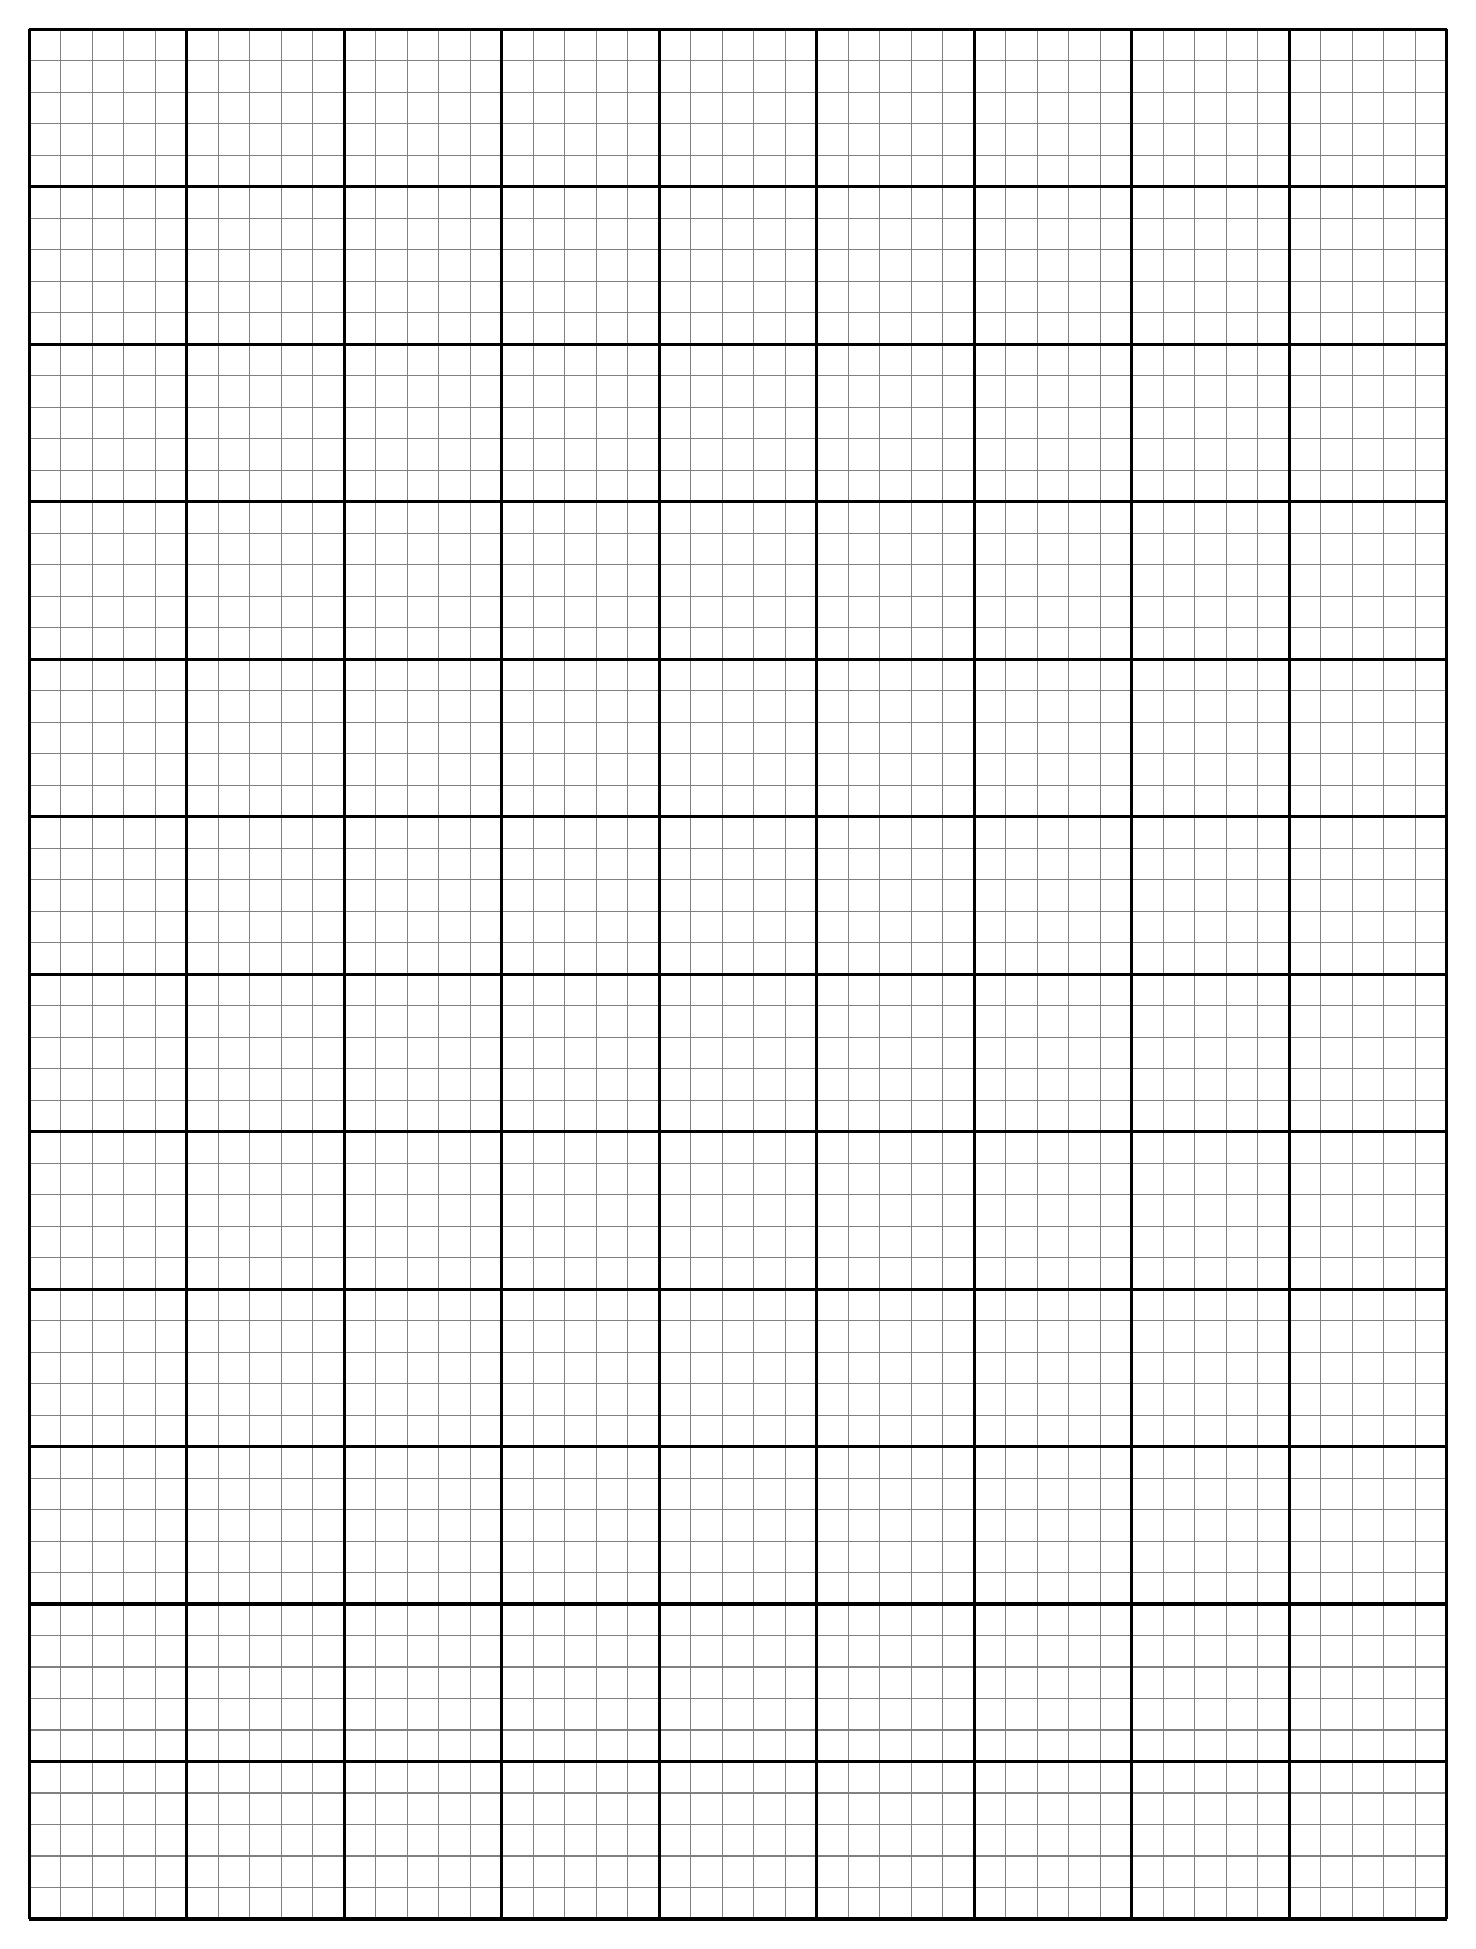
\begin{tikzpicture}[every node/.style={minimum size=1cm-\pgflinewidth, outer sep=10pt}, scale=2]
    \draw[step=0.2cm,color=gray] (0,0) grid (9,12);
    \draw[step=1cm,color=black,line width=0.4mm] (0,0) grid (9,12);
    \end{tikzpicture}
    \newpage
}

\scriptsize
\tableofcontents
\section{最短路徑}
    \subsection{basic}
        \lstinputlisting{Contents/最短路徑/basic.cpp}

\section{圖論}
    \subsection{凸包問題}
        \lstinputlisting[language={[ISO]C++}]{Contents/圖論/convexhull.code}
        \lstinputlisting{Contents/圖論/convexhull.cpp}

\section{數學}
    \subsection{公式}
        \begin{itemize}
    \item 錯排公式 :  ($n$個人中，每個人皆不再原來位置的組合數): \\
      $dp[0]=1;dp[1]=0;$\\
      $dp[i]=(i-1)*(dp[i-1]+dp[i-2])$;
    \item 一個環上相鄰顏色不同的染色數量 : \\
      $f(n,k) = (k-1)^n + (-1)^n(k-1)$\\
      n是點的數量，k是顏色的數量
    \item Kőnig 定理：\\
      在二分圖中\\
      最大匹配 \equiv 最小點覆蓋\\
      最小邊覆蓋 \equiv 最大獨立集\\
      點數 \equiv 最大匹配 $+$ 最小邊覆蓋\\
      點數 \equiv 最大獨立集 $+$ 最小點覆蓋

\end{itemize}

\end{document}
